\documentclass[a4paper]{article}

\usepackage{color}
\usepackage{xurl}
\usepackage[T2A]{fontenc}
\usepackage[utf8]{inputenc}
\usepackage{csquotes}
\usepackage{graphicx}
\usepackage{subfigure}
\usepackage{float}
\usepackage[english,serbian]{babel}
\usepackage{listings}
\usepackage{algorithm}
\usepackage{algpseudocode}
\usepackage{amsthm}
\usepackage{amsmath}

\usepackage[unicode]{hyperref}
\hypersetup{colorlinks,citecolor=green,filecolor=green,linkcolor=blue,urlcolor=blue}

\newtheorem{theorem}{Theorem}[section]
\newtheorem{lemma}[theorem]{Lema}

\floatname{algorithm}{Algoritam}

\title{\textit{Beam Stack Search} algoritam pretrage u okviru alata za simboličko izvršavanje KLEE\\ \small{Seminarski rad u okviru kursa\\Verifikacija softvera\\Matematički fakultet}}
\author{Aleksandar Stefanović, 1021/2023 \and Petar Đorđević, 1088/2022}

\begin{document}

\maketitle

\begin{abstract}

Jedan od osnovnih problema simboličkog izvršavanja kao tehnike verifikacije softvera je eksplozija broja stanja, tj. putanja kojima izvršavanje programa može da teče. Zbog toga, praktično je nemoguće izvršiti potpunu pretragu svih putanja izvršavanja programa, pa alati za simboličko izvršavanje, poput alata KLEE, koriste različite heurističke pristupe za izbor podskupa putanja za istraživanje.

Ovaj rad je posvećen implementaciji \textit{Beam Stack Search} algoritma pretrage u okviru alata za simboličko izvršavanje KLEE, modifikacije \textit{Beam Search} algoritma koji svoje primene najčešće nalazi u oblasti mašinskog učenja, konkretno u obradi prirodnog jezika i mašinskog prevođenja. Eksperimentalnom evaluacijom pokazujemo da se \textit{Beam Stack Search} algoritam u nekim realnim primerima ponaša bolje od podrazumevanog algoritma pretrage alata KLEE.

\end{abstract}

\tableofcontents

\newpage

\section{Uvod}

Simboličko izvršavanje u svom osnovnom obliku predstavlja tehniku statičke verifikacije programa, tj. verifikacije programa bez njegovog pokretanja, u kojoj se umesto konkretnog stanja programa tokom izvršavanja prati njegovo simboličko stanje \cite{SymExec-King-10.1145/360248.360252}, u cilju otkrivanja grešaka, automatskog generisanja testova sa velikom pokrivenošću koda i slično. Ovo podrazumeva praćenje simboličkih vrednosti promenljivih koje se javljaju u programu, kao i tzv. uslova putanja - logičkih formula nad simboličkim vrednostima tih promenljivih koje moraju da budu zadovoljene da bi izvršavanje stiglo do neke tačke u programu.

Svaka naredba kontrole toka, poput naredbi grananja ili petlji, može prouzrokovati više putanja izvršavanja programa. Ove putanje, zajedno sa pridruženim uslovima putanja i simboličkim vrednostima promenljivih, indukuju simboličko stablo izvršavanja programa. Osim za najtrivijalnije programe, simboličko stablo izvršavanja je nemoguće u potpunosti istražiti. Simboličko stablo izvršavanja program koji sadrži samo $30$ naredbi grananja, zanemarujući moguće nedostižne putanje, sadržalo bi $2^{30}$ različitih putanja izvršavanja. Ukoliko program sadrži i petlje, njegovo stablo izvršavanja bi potencijalno bilo i beskonačno veliko (ukoliko i sam uslov prekida petlje ima simboličku vrednost).

Upravo eksplozija broja stanja u simboličkom stablu izvršavanja je jedan od glavnih problema sa kojim se susreću alati za simboličko izvršavanje. Neke od tehnika koje alati koriste da bi umanjili efekat ovog problema su odsecanje nedostižnih putanja, spajanje stanja, zadavanje preduslova i aproksimacija petlji \cite{SurveySymExec-CSUR18}. Međutim, čak i uz primenu ovih tehnika, najčešće nije moguće eliminisati dovoljan broj stanja da bi se efikasno istražilo celokupno simboličko stablo izvršavanja, pa je od velike važnosti izbor stanja, tj. putanja, za ispitivanje.

Izbor narednog stanja za ispitivanje zavisi od primenjene strategije za obilazak puteva. Dve osnovne strategije su \textit{DFS}, tj. pretraga u dubinu, i \textit{BFS}, tj. pretraga u širinu. Iako imaju svoje primene, obe strategije imaju svoje mane - pretraga u dubinu ima tendenciju zaglavljivanja u \enquote{dubokim} putanjama indukovanih petljama ili rekurzijom, dok pretraga u širinu povlači izuzetno veliko memorijsko zauzeće usled potrebe za istovremenim čuvanjem čitavog nivoa, tj. sloja čvorova simboličkog stabla izvršavanja. Postoje i hibridne tehnike između ova dva pristupa, poput algoritma \textit{BFS-DFS} \cite{BFS/DFS-StrahinjaStanojevic}. Često se primenjuju i tehnike koje koriste randimozovane varijante algoritama pretrage, gde se stanjima koja imaju neku dobru osobinu može dodeliti prednost prilikom izbora, poput algoritma koji podrazumevano koristi alat za simboličko izvršavanje \verb|KLEE| \cite{KLEE-paper-10.5555/1855741.1855756}.

U nastavku rada će biti predstavljena upotreba \textit{Beam Stack Search} algoritma pretrage, kao i njegova implementacija u okviru alata za simboličko izvršavanje \verb|KLEE|. Na kraju, biće izvršena uporedna analiza performansi ovog algoritma sa podrazumevanim algoritmom koji koristi alat \verb|KLEE|.

\section{Opis algoritma}

Algoritam \textit{Beam Stack Search} \cite{BeamStackSearch-10.5555/3037062.3037074} predstavlja proširenje heurističkog algoritma pretrage \textit{Beam Search}, pa će u nastavku prvo biti opisan ovaj algoritam. Iako u opštem slučaju ovi algoritmi imaju mogućnost obilaska proizvoljnog grafa, u nastavku rada će se, zbog potreba u simboličkom izvršavanju, razmatrati samo obilazak stabla.

\subsection{\textit{Beam Search} algoritam pretrage}

Algoritam pretrage \textit{Beam Search}, nadalje \textit{BS} algoritam, svoje najveće primene nalazi u oblasti mašinskog učenja, konkretno u obradi prirodnog jezika i mašinskog prevođenja \cite{HarpySpeechRecognitionSystem, BeamSearchStrategiesForNeuralMachineTranslation, BestFirstBeamSearch}. Međutim, ideje koje on uvodi se mogu primeniti i u simboličkom izvršavanju. Naime, \textit{BS} algoritam, po cenu gubitka kompletnosti pretrage, heurističkim pristupom brzo i uz malu memorijsku potrošnju pronalazi dobre, po nekoj izabranoj meri kvaliteta, putanje u težinskom grafu. U kontekstu simboličkog izvršavanja, ova ideja se može primeniti na pronalaženje putanja koje, na primer, maksimizuju pokrivenost koda.

Algoritam kao parametar prihvata ceo broj $w$, tj. širinu pretrage, i zasnovan na \textit{BFS} pretrazi, sa modifikacijom da na svakom nivou stabla pretrage zadržava samo $w$ najboljih čvorova (najveće ili najmanje težine, zavisno od izabrane mere kvaliteta čvora), a ostale čvorove odbacuje. Primer izvršavanja za $w = 2$ nad stablom gde se prednost daje čvorovima veće težine prikazan je na slici \ref{fig:beam_search}. Zeleni čvorovi označavaju čvorove izabrane za pretragu, crveni čvorove koji su odbačeni, a svetlo crveni čvorove koji, kao potomci odbačenih čvorova, nisu ni razmatrani.

\begin{figure}[h!]
    \centering
    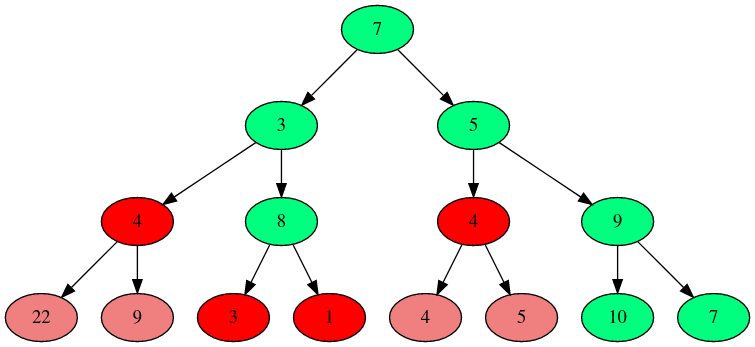
\includegraphics[width=\linewidth]{ilustracije/beam_search_primer.png}
    \caption{Izvršavanje \textit{BS} algoritma nad stablom za širinu pretrage $w = 2$}
    \label{fig:beam_search}
\end{figure}

Pošto se na svakom nivou stabla zadržava samo $w$ čvorova, a prethodno posećeni čvorovi se ne pamte, memorijska složenost ovog algoritma pretrage je $O(w)$, tj. ne zavisi od veličine stabla. Međutim, problem u ovom pristupu je to što će samo $w$ putanja biti u potpunosti istraženo, pod pretpostavkom da su one konačne dužine. U kontekstu simboličkog izvršavanja, ovo bi dovelo do gubitka saglasnosti analize. Da bi se ovaj problem rešio, potrebno je izvršiti modifikaciju algoritma, koja je data u vidu \textit{Beam Stack Search} algoritma pretrage.

\subsection{\textit{Beam Stack Search} algoritam pretrage}

Algoritam \textit{Beam Stack Search}, nadalje \textit{BSS}, prvi put je opisan u radu \cite{BeamStackSearch-10.5555/3037062.3037074} i predstavlja nadogradnju osnovnog \textit{Beam Search} algoritma koja rešava prethodni problem odbacivanja potencijalno važnih putanja izvršavanja, ali po cenu povećane memorijske složenosti. Naime, osnovna ideja \textit{BSS} algoritma je u tome da se, umesto odbacivanja, neposećena stanja čuvaju za kasniju obradu u posebno uređenoj stek strukturi. Stek je uređen po nivoima - čvorovi na proizvoljnom nivou stabla koji su razmatrani, ali ne i izabrani za obradu, se postavljaju kao jedan nivo čvorova na steku. U trenutku kada bi standardna \textit{Beam Search} pretraga stigla do kraja stabla, sa vrha steka se uzima jedan nivo čvorova i nastavlja se sa pretragom. Algoritam je prikazan pseudokodom \ref{alg:tree_beam_stack_search}.

\begin{algorithm}
    \begin{algorithmic}[1]
            \Procedure{BSS}{Tree t, Int w}
                \State Vec<Node> currentLevel = \{t.root()\}
                \State Vec<Node> nextLevel = \{\}
                \State Stack<Vec<Node>{>} beamStack = \{\}
                \While {not currentLevel.empty()}
                    \For {Node n in currentLevel}
                        \State visit(n)
                        \State nextLevel.append(t.adjacent(n))
                    \EndFor
                    \State nextLevel.sort()
                    \State Int beamWidth = min(nextLevel.size(), w)
                    \State currentLevel = nextLevel[0 : beamWidth]
                    \If {beamWidth != nextLevel.size()}
                        \State beamStack.push(nextLevel[beamWidth : nextLevel.size()])
                    \EndIf
                    \State nextLevel.clear()
                    \If {currentLevel.empty() and not beamStack.empty()}
                        \State currentLevel = beamStack.top()
                        \State beamStack.pop()
                    \EndIf
                \EndWhile
            \EndProcedure
    \end{algorithmic}
    \caption{Tree Beam Stack Search}
    \label{alg:tree_beam_stack_search}
\end{algorithm}

Upotreba steka sa neposećenim čvorovima garantuje da će svi čvorovi stabla u nekom trenutku biti posećeni, ali njegovo održavanje zahteva dodatnu memoriju u odnosu na klasičan \textit{Beam Search} algoritam. Ukoliko pretpostavimo da je stablo nad kojem se algoritam izvršava binarno, što i jeste validna pretpostavka za osnovni slučaj simboličkog stabla izvršavanja, može se pokazati da je memorijska složenost algoritma ograničena sa dubinom stabla i zadatim parametrom širine pretrage $w$.

\begin{lemma}
Ukoliko se algoritam \textit{Beam Stack Search} primenjuje nad binarnim stablom, memorijska složenost algoritma je $O(dw)$, gde $d$ predstavlja dubinu stabla, a $w$ je zadati parametar širine pretrage.
\end{lemma}

\begin{proof}
Za dokaz je dovoljno pokazati da je (1) veličina svakog nivoa čvorova na steku najviše $w$ i (2) na steku je u svakom trenutku najviše $d$ nivoa čvorova.
\begin{enumerate}
    \item Posmatrajmo skup izabranih čvorova u $i$-toj iteraciji algoritma \ref{alg:tree_beam_stack_search}, u oznaci $currentLevel$. Pre ulaska u petlju, ovaj skup sadrži samo koren stabla, te je njegova kardinalnost jednaka $card(currentLevel) = 1$. U $i-toj$ iteraciji petlje, skup čvorova $currentLevel$ se ažurira tako što se od njima susednih čvorova, u oznaci $nextLevel$, bira $min(w, card(nextLevel))$ njih. Prema tome, važi da je $card(currentLevel) \leq w$ u svakoj iteraciji petlje. Usled uslova da je stablo binarno, dodatno važi i $card(nextLevel) \leq 2 \cdot card(currentLevel) \leq 2w$. Pošto se na stek dodaju skupovi čvorova veličine $card(nextLevel) - w$, iz prethodnog važi da će se na steku u svakom trenutku nalaziti samo skupovi čvorova veličine manje ili jednake od $w$.

    \item Dovoljno je primetiti da nivoi na steku, počev od njegovor vrha, odgovaraju strogo opadajućem redosledu nivoa u stablu, gde najmanji nivo ima koren stabla. Naime, svakim ponovnim pokretanjem pretrage od nekog nivoa na steku se taj nivo skida sa steka, a dalja pretraga do ponovnog pokretanja od nekog nivoa sa steka teče strogo niz stablo, pa sledi da je nivo koji odgovara svakom skupu čvorova koji se dodaje na stek strogo manji od onog koji je prethodno izbačen sa steka, kao i od onog koji je prethodno dodat na stek. Pošto stablo ima najviše $d$ nivoa, sledi da se na steku u svakom trenutku može naći najviše $d$ nivoa čvorova.
\end{enumerate}
\end{proof}

Ovako ograničena memorijska složenost sprečava prebrzo zauzeće memorije, kao što je to slučaj kod klasičnog $BFS$ algoritma, ali pritom zadržava mogućnost šireg prostora pretrage i istovremenog praćenja više potencijalno zanimljivih putanja pomoću podesivog parametra širine pretrage $w$. Zapravo, za vrednost parametra $w = 1$, algoritam bi se ponašao kao $DFS$ algoritam pretrage, pri čemu se u svakom koraku bira bolji čvor za nastavak pretrage, dok bi se za dovoljno veliko $w$, vrednosti veće ili jednake širini celokupnog stabla, ponašao kao $BFS$ algoritam. Dodatno, izbor čvorova za posetu prema nekoj izabranoj meri kvaliteta omogućava brži pronalazak kvalitetnih putanja, što bi u kontekstu simboličkog izvršavanja moglo da podrazumeva putanje čije izvršavanje osigurava veliki stepen pokrivenosti koda.

\section{Implementacija u okviru alata za simboličko izvršavanje KLEE}

Implementacija \textit{BSS} algoritma pružena je kroz klasu \verb|BeamSearcher|, specijalizaciju apstraktne klase \verb|Searcher| - bazne klase svih algoritama pretrage u okviru alata KLEE. Potpuna implementacija dostupna je na repozitorijumu \cite{Projekat}. Klasa \verb|BeamSearcher| implementira naredne čisto virtualne metode iz klase \verb|Searcher|:

\begin{itemize}
    \item \textbf{selectState:} Ova metoda bira jedno stanje za dalje istraživanje. U kontekstu \textit{BSS} algoritma, bira se prvo stanje u trenutnom sloju.

    \item \textbf{update:} Ova metoda obaveštava pretraživač o novim ili uklonjenim stanjima. Koristi se za ažuriranje slojeva pretrage nakon što su stanja razgranata ili uklonjena.

    \item \textbf{empty:} Ova metoda proverava da li su sva stanja istražena, tj. da li pretraživač više nema stanja za istraživanje.
\end{itemize}

\subsection{Modifikacija u implementaciji algoritma}

U implementaciji algoritma uvedena je modifikacija u odnosu na prethodno opisanu \textit{BSS} pretragu - dodatni parametar, \verb|beamStackSwapLimit|, koji je uveden kako bi se izbeglo zaglavljivanje u lokalnim maksimumima tokom pretrage. Ovaj parametar omogućava pretraživaču da, nakon određenog broja posećenih stanja u kojima nije pronađeno novo pokrivanje (\verb|statesSinceLastCoveredNew|), pretragu nastavi od sloja sa dna steka, čime se postiže vraćanje pretrage na više nivoe stabla. Postavljanjem vrednosti parametra \verb|beamStackSwapLimit| na 0, algoritam se ponaša kao standardna \textit{BSS} pretraga.

Iako se ovom modifikacijom gubi garancija memorijske složenosti od $O(dw)$, eksperimentalno se pokazalo da nema značajan negativan uticaj na performanse algoritma dok istovremeno povećava njegovu robusnost u situacijama sa kompleksnim pretraživačkim prostorima.

\subsection{Mera kvaliteta pri izboru stanja}

Mera kvaliteta za izbor stanja za naredni nivo pretrage zasnovana je na istoj strategiji kao i podrazumevani \emph{nurs:covnew} (\emph{Non-Uniform Random Search}) algoritam. Ova mera kombinuje dve komponente:

\begin{enumerate}
\item Minimalna udaljenost do najbliže nepokrivene instrukcije u grafu kontrole toka.
\item Broj instrukcija izvršenih od poslednje pokrivene nove instrukcije.
\end{enumerate}

Algoritam maksimizuje pokrivenosti koda tako što bira stanja koja verovatnije vode do do tog trenutka nepokrivenih delova programa. Pošto manja vrednost za obe komponente daje veći prioritet stanju, one se invertuju kako bi se postigao željeni efekat.

\subsection{Pokretanje algoritma u okviru alata KLEE}

Alat KLEE omogućava korisnicima da prilagode način pretrage kroz veliki broj različitih opcija. Za podešavanje parametara \verb|BeamSearcher| pretrage, pružene su dve nove opcije:

\begin{enumerate}
    \item \textbf{{-}{-}beam-width}: Ova opcija postavlja širinu pretrage, tj. broj stanja koja se zadržavaju za dalje istraživanje u svakom sloju pretrage. Širina pretrage određuje koliko različitih grana se istražuje u jednom trenutku. Podrazumevana vrednost za ovu opciju je 256.
    \item \textbf{{-}{-}beam-stack-swap-limit}: Ova opcija određuje maksimalni broj stanja koja će biti posećena u nizu bez pokrivanja nove instrukcije pre nego što se pretraga vrati na najranije odložena stanja, uzimanjem sloja sa dna steka za dalju pretragu. Postavljanjem vrednosti na 0, ova opcija se isključuje. Podrazumevana vrednost je 1 000 000.
\end{enumerate}

Za pokretanje alata KLEE koristeći \verb|BeamSearcher| pretragu sa specifičnim vrednostima za širinu pretrage 128 i maksimalno 500 000 stanja bez pokrivanja nove instrukcije pre prelaska na ranija stanja, može se koristiti naredna komanda:

\begin{verbatim}
klee --searcher=beam \
     --beam-width=128 \
     --beam-stack-swap-limit=500000 \
     /putanja/do/programa.bc
\end{verbatim}

\section{Eksperimentalna evaluacija algoritma}

Radi utvrđivanja performansi \textit{Beam Stack Search} algoritma, sprovedeni su eksperimenti nad slučajno odabranim podskupom \verb|GNU Coreutils| alata \cite{GNUCoreutils}, konkretno nad alatima \verb|printf|, \verb|mkdir|, \verb|sha256sum|, \verb|touch| i \verb|sort|. Nad svakim od njih je izvršeno po jedno pokretanje \textit{Beam Stack Search} pretrage i podrazumevane pretrage alata KLEE - isprepletane \textit{nurs:covnew} i \textit{Random Path} pretrage.

Kako bi se omogućila adekvatna uporedivost rezultata između \textit{Beam Stack Search} i podrazumevanog algoritma pretrage, sva testiranja su sprovedena u konzistentnim uslovima sa parametrima što sličnijim onim koji su korišćeni u originalnom radu o alatu KLEE \cite{KLEE-paper-10.5555/1855741.1855756, KLEEExperiments}. \textit{Beam Stack Search} algoritam je pokretan sa podrazumevanim vrednostima parametara \verb|--beam-width| od 256 i \verb|--beam-stack-swap-limit| od 1 000 000. Kao i u originalnom eksperimentu, sve iteracije su trajale po jedan sat, a memorija je bila ograničena na 1GB.

Za deo testiranih programa, \textit{Beam Stack Search} algoritam pokazuje blago poboljšanje u pokrivenosti instrukcija u odnosu na podrazumevani algoritam pretrage. Na primer, kod programa \verb|printf|, \textit{BSS} algoritam postiže 49.81\% pokrivenosti instrukcija, što je za 2.46\% više u odnosu na podrazumevani algoritam. Slično tome, \verb|sha256sum| beleži poboljšanje od 1.31\% sa \textit{BSS} algoritmom.

Međutim, postoji izuzetak kod programa \verb|sort|, gde \textit{BSS} algoritam značajno zaostaje sa pokrivenošću od 26.54\%, što je za 9.83\% manje u poređenju sa podrazumevanim algoritmom. Za preostala dva programa beleže se slični rezultati. Rezultati se mogu videti na slici \ref{fig:icov_comparison} i u tabeli \ref{tab:icov_comparison}.

\begin{figure}[h!]
    \centering
    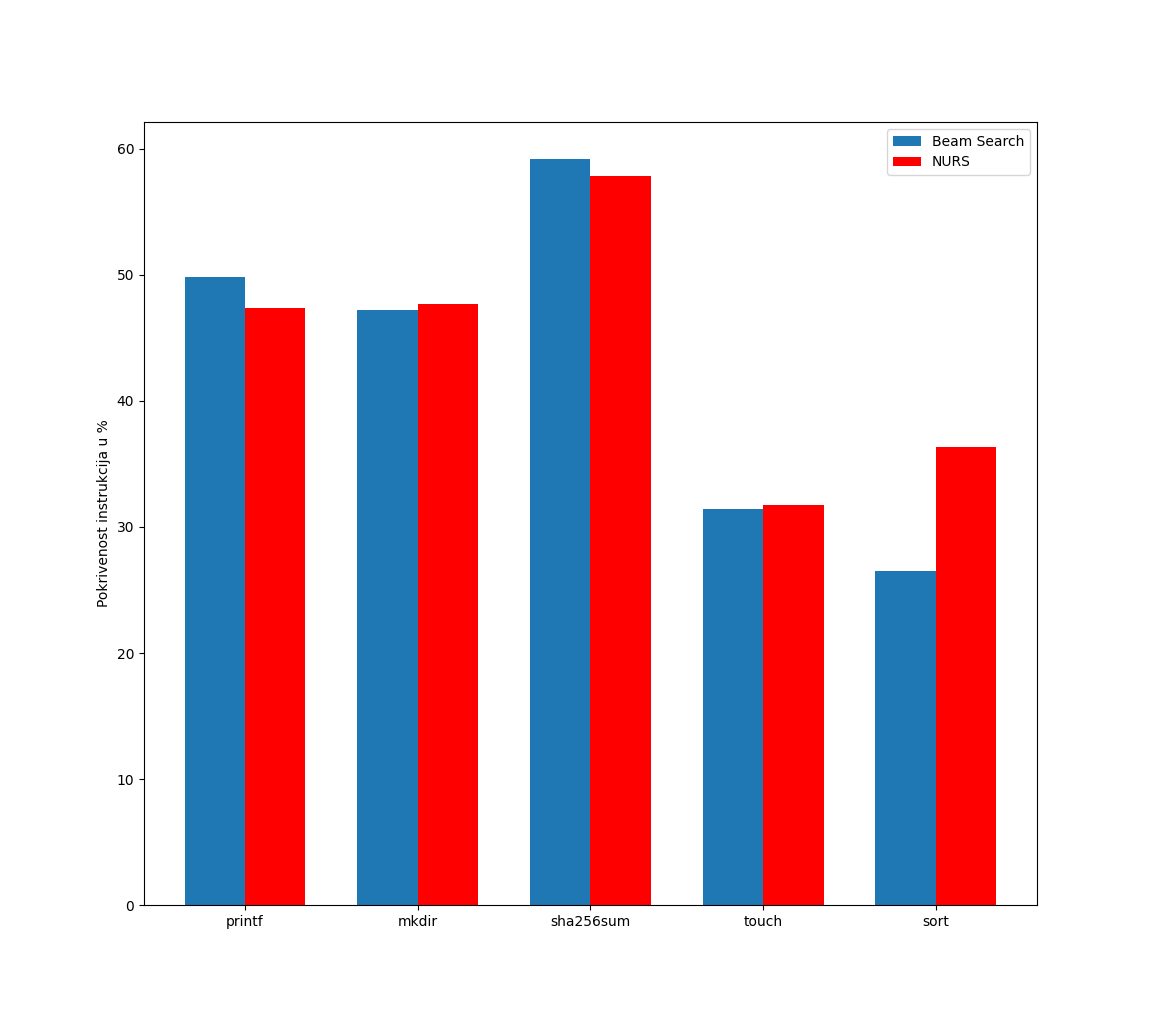
\includegraphics[width=\linewidth]{ilustracije/ICov.png}
    \caption{Poređenje pokrivenosti instrukcija za \textit{Beam Stack Search} i podrazumevani algoritam pretrage}
    \label{fig:icov_comparison}
\end{figure}

\begin{table}[h!]
\centering
\begin{tabular}{|l|c|c|c|}
\hline
\textbf{Program} & \textbf{nurs ICov (\%)} & \textbf{beam ICov (\%)} & \textbf{Razlika ICov (\%)} \\ \hline
\texttt{printf} & 47.35 & 49.81 & 2.46 \\ \hline
\texttt{mkdir} & 47.71 & 47.18 & -0.53 \\ \hline
\texttt{sha256sum} & 57.85 & 59.16 & 1.31 \\ \hline
\texttt{touch} & 31.71 & 31.44 & -0.27 \\ \hline
\texttt{sort} & 36.37 & 26.54 & -9.83 \\ \hline
\end{tabular}
\caption{Poređenje pokrivenosti instrukcija za \textit{Beam Stack Search} i podrazumevani algoritam pretrage}
\label{tab:icov_comparison}
\end{table}

\begin{figure}[h!]
    \centering
    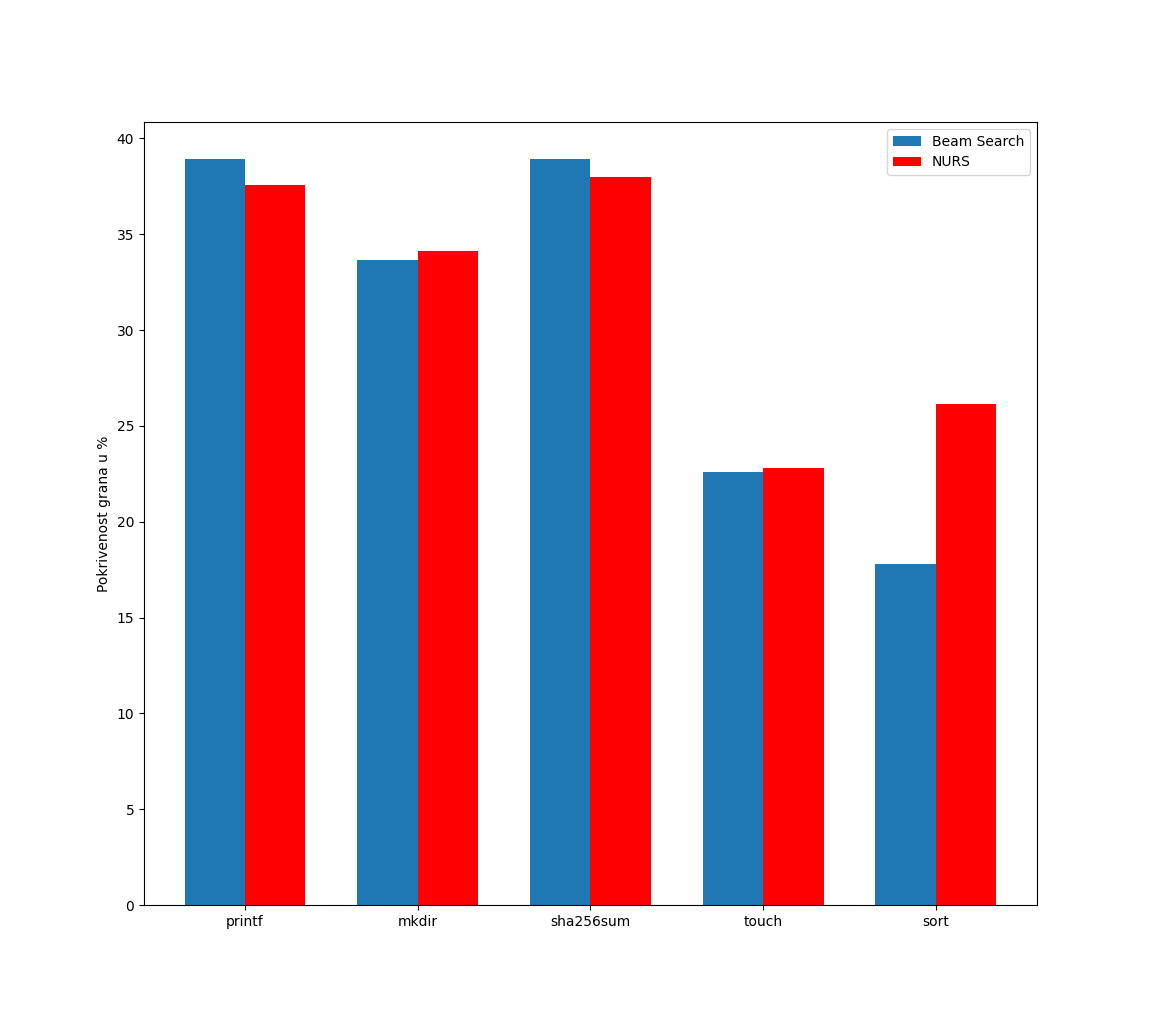
\includegraphics[width=\linewidth]{ilustracije/BCov.png}
    \caption{Poređenje pokrivenosti grana za nurs i beam algoritme}
    \label{fig:bcov_comparison}
\end{figure}

Slično kao i kod pokrivenosti instrukcija, \textit{Beam Stack Search} algoritam pokazuje poboljšanje u analizi \verb|printf| i \verb|sha256sum| programa i sličan rezultat u \verb|mkdir| i \verb|touch| kada je reč o pokrivenosti grana. Na primer, kod programa \verb|printf|, \textit{BSS} algoritam povećava pokrivenost grana za 1.32\% u poređenju sa podrazumevanim algoritmom. Takođe, kod \verb|sha256sum|, \textit{BSS} algoritam beleži blago poboljšanje od 0.91\%. Opet, kod programa \verb|sort|, primećujemo značajno smanjenje pokrivenosti grana, gde \textit{BSS} algoritam postiže samo 17.80\%, što je za 8.35\% manje od podrazumevanog algoritma. Rezultati se mogu videti na slici \ref{fig:bcov_comparison} i u tabeli \ref{tab:bcov_comparison}.

\begin{table}[h!]
\centering
\begin{tabular}{|l|c|c|c|}
\hline
\textbf{Program} & \textbf{nurs BCov (\%)} & \textbf{beam BCov (\%)} & \textbf{Razlika BCov (\%)} \\ \hline
\texttt{printf} & 37.59 & 38.91 & 1.32 \\ \hline
\texttt{mkdir} & 34.11 & 33.67 & -0.44 \\ \hline
\texttt{sha256sum} & 38.00 & 38.91 & 0.91 \\ \hline
\texttt{touch} & 22.83 & 22.58 & -0.25 \\ \hline
\texttt{sort} & 26.15 & 17.80 & -8.35 \\ \hline
\end{tabular}
\caption{Poređenje pokrivenosti grana vrednosti za nurs i beam algoritme}
\label{tab:bcov_comparison}
\end{table}

Nad programima \verb|printf|, \verb|sha256sum| i \verb|sort| dodatno je pokrenuta i analiza sa \textit{BSS} algoritmom bez modifikacije sa uzimanjem sloja stanja sa dna steka, tj. sa vrednosti 0 za parametar \verb|--beam-stack-swap-limit|. U sva tri slučaja, dobijena pokrivenost, kako instrukcija, tako i grana, je bila manja nego sa modifikacijom (47.24\%, 56.20\% i 26.52\% za pokrivenost instrukcija i 37.48\%, 36.30\% i 17.78\% za pokrivenost grana, redom za \verb|printf|, \verb|sha256sum| i \verb|sort|).

\section{Zaključak}

Eksperimentalni rezultati pokazuju da \textit{Beam Stack Search} algoritam u velikom broju slučajeva postiže veoma dobre rezultate u kontekstu nivoa pokrivenosti koda - najčešće približno ili čak bolje od podrazumevanog algoritma pretrage alata KLEE. Međutim, zaglavljivanje u pretrazi programa velike složenosti je i dalje moguće, što se može videti iz loših rezultata prilikom analize programa \verb|sort|. Jedan moguć način rešavanja ovog problema je isprepletano pokretanje nekog od nasumičnih algoritama pretrage, poput \textit{Random Path Selection} algoritma, zajedno sa \textit{Beam Stack Search} pretragom.

Potencijalno poboljšanje algoritma \textit{Beam Stack Search} u kojem se bi se dalje istraživanje moglo kretati je uvođenje nedeterminizma u sam algoritam radi izbegavanja zaglavljivanja, na primer izborom nasumičnog nivoa stanja sa steka umesto isključivo sa dna prilikom korišćenja \verb|--beam-stack-swap-limit| modifikacije. Dodatno, potrebno je sprovesti dalja istraživanja o ponašanju pretrage u zavisnosti od karakteristika ulaznog programa i vrednosti parametara \verb|--beam-width| i \verb|--beam-stack-swap-limit|.

\addcontentsline{toc}{section}{Literatura}
\appendix
\bibliography{literatura}
\bibliographystyle{plain}

\end{document}
